\documentclass{article}
\usepackage{graphicx}

\graphicspath{ {../graphs/} }
\title{Constraint-Satisfaction EA}
\author{Bryan A. Asher}
\date{\today}
\begin{document}
Bryan A. Asher

baa522@mst.edu

CS5401 FS2018 Assignment 1c

\maketitle
% \begin{flushright}
% Bryan A. Asher

% baa522@mst.edu

% CS5401 FS2018 Assignment 1c

% \end{flushright}

\section{Methodology}
All T-test preformed using a two-tailed distribution, a two-sample unequal variance (heteroscedastic) test is performed, the alpha parameter is 0.05 and each sample size is fifty fitnesses. The null hypothesis for all test is that the population mean fitnesses for the first sample is equal to the second sample. All comparisons between runs of the EA are kept as similar as possible only changing the parameter of interest. All data is in terms of average population fitness per number of evaluations.

\section{Analyzing Improvement in a Constraint-Satisfaction EA Employing a Penalty Function}

	\subsection{Assigned Board}

		A constraint-satisfaction EA employing a penalty function offers better results than a basic EA, 
		considering the T-test p-value  of 0; when compared to a repair function the T-test p-value of 0.0005 shows that 	the repair function preforms better.
		\begin{figure}[!htb]
		\centering
		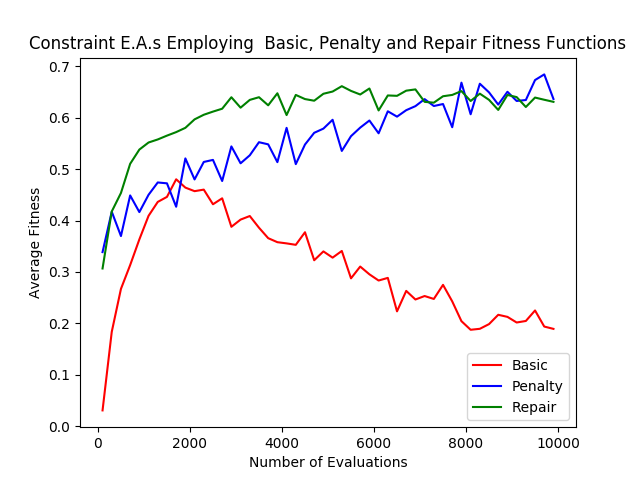
\includegraphics[scale=0.4]{q1_assigned_board_penalty_vs_basic_vs_repair.png}
		% \caption{Assigned Board}
		\end{figure}
		
		\begin{center}
		\begin{tabular}{ || c | c | c | c ||}
		\hline
		       & Basic & Penalty & Repair \\ 
		 \hline\hline
		 Average & 0.3070432432	& 0.5558156757 & 0.6092613514 \\ 
		 \hline
		 Standard Deviation &	0.09853981983 &	0.08217763332 &	0.06606127677 \\
		 \hline
		 variance &	0.009710096093 &	0.006753163418 &	0.004364092289 \\
		 \hline
		 T-test &	0	& &	0.0005390132579 \\
		 \hline
		\end{tabular}
		\end{center}
		
		\subsection{Random Boards}

			A constraint-satisfaction EA employing a penalty function offers equivalent results to a basic EA, 
			considering the T-test p-value  of 0.19; when compared to a repair function the T-test p-value of 0 shows that 	the 		repair function preforms better.
			\begin{figure}[!htb]
			\centering
			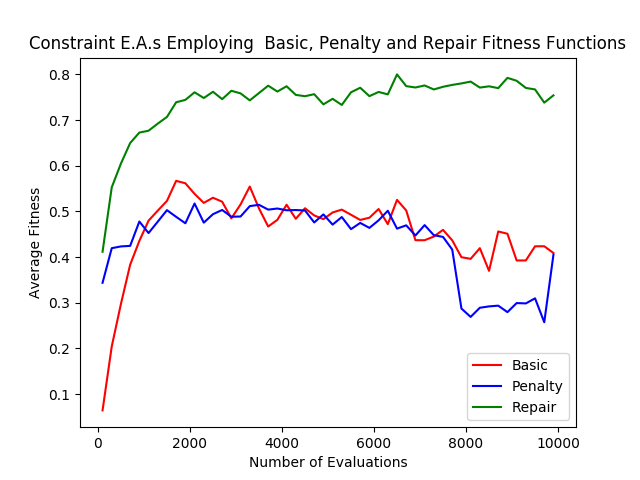
\includegraphics[scale=0.4]{q1_random_boards_penalty_vs_basic_vs_repair.png}
			% \caption{Assigned Board}
			\end{figure}
			
			\begin{center}
			\begin{tabular}{ || c | c | c | c ||}
			\hline
			       & Basic & Penalty & Repair \\ 
			 \hline\hline
			 Average & 0.45654198 &	0.4347807821 & 0.7401661915	 \\ 
			 \hline
			 Standard Deviation &	0.08695585547 &	0.08118205986 &	0.06595359204	 \\
			 \hline
			 variance &	0.007561320801 &	0.006590526844 &	0.004349876303 \\
			 \hline
			 T-test &	0.1988983448	& &	0 \\
			 \hline
			\end{tabular}
			\end{center}
\clearpage


\section{Comparing EAs Employing Forced Validity and Uniform Random Initialization}

	\subsection{Assigned Board}

		\subsubsection{Basic Fitness}
			Both configurations preformed equivalently bad. Uniform random initialization preformed
			very poorly for basic fitness, if the few fit individuals in a population 
			do not get picked to be parents, the average fitness falls to zero quickly.

			\begin{figure}[!htb]
			\centering
			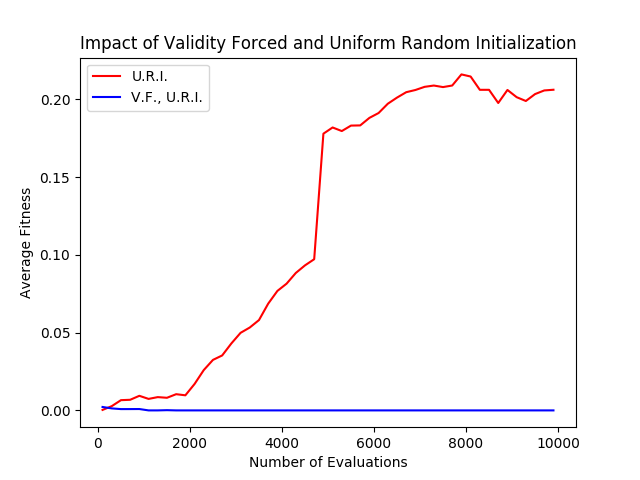
\includegraphics[scale=0.4]{q2_assigned_board_basic_ur_vs_vfur.png}
			% \caption{Assigned Board}
			\end{figure}
			\begin{center}
			\begin{tabular}{ || c | c | c | c ||}
			\hline
			       & F.V. and U.R. & U.R.\\ 
			 \hline\hline
			 Average & 0.1215887387 &	0.0001240540541 \\ 
			 \hline
			 Standard Deviation &	0.08535172176	& 0.000402820311
					 \\
			 \hline
			 variance &	0.007284916408 &	0.000000162264203 \\
			 \hline
			 T-test &	0	& \\
			 \hline
			\end{tabular}
			\end{center}
\clearpage
		\subsubsection{Penalty Fitness}
			Uniform random initialization preformed less poorly for Penalty fitness, the added
			genetic diversity help slow fitness degradation. But, again, both configurations
			preformed equivalently poor.

			\begin{figure}[!htb]
			\centering
			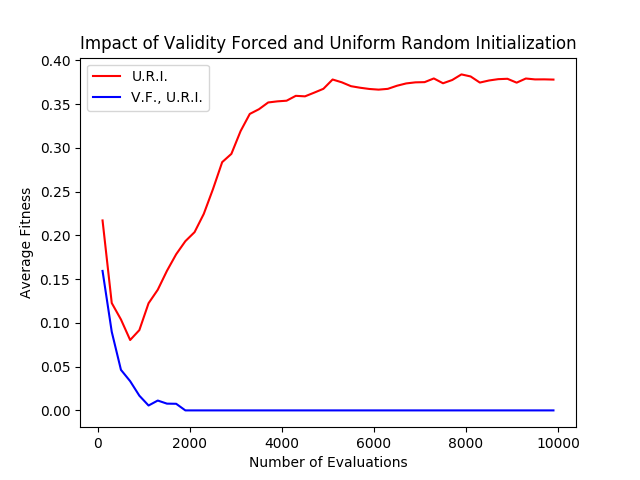
\includegraphics[scale=0.4]{q2_assigned_board_penalty_ur_vs_vfur.png}
			% \caption{Assigned Board}
			\end{figure}
			\begin{center}
			\begin{tabular}{ || c | c | c | c ||}
			\hline
			       & F.V. and U.R. & U.R.\\ 
			 \hline\hline
			 Average & 0.3111825676 &	0.007559121622 \\ 
			 \hline
			 Standard Deviation &	0.09619133965	& 0.02651297888\\
			 \hline
			 variance &	0.009252773823 &	0.0007029380489 \\
			 \hline
			 T-test &	0	& \\
			 \hline
			\end{tabular}
			\end{center}
	

		\subsubsection{Repair Fitness}
			Both configurations with repair preformed equivalently well. These configurations
			did not share the same loss of fitness as the other configurations due to the 
			volume of fit individuals.
			\begin{figure}[!htb]
			\centering
			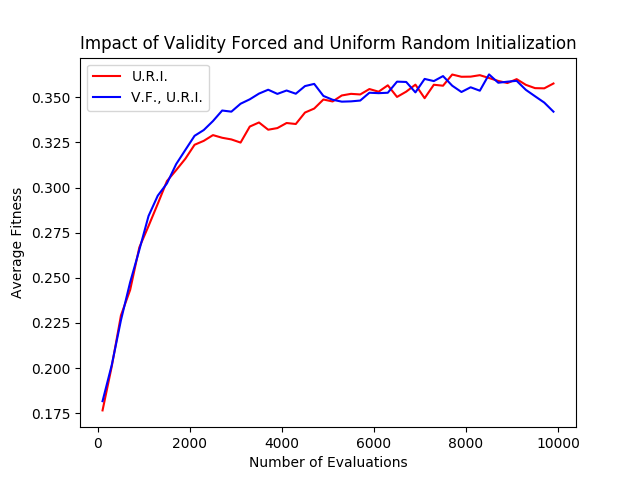
\includegraphics[scale=0.4]{q2_assigned_board_repair_ur_vs_vfur.png}
			% \caption{Assigned Board}
			\end{figure}
			\begin{center}
			\begin{tabular}{ || c | c | c | c ||}
			\hline
			       & F.V. and U.R. & U.R.\\ 
			 \hline\hline
			 Average & 0.3302622748 &	0.3339137838 \\ 
			 \hline
			 Standard Deviation &	0.04177146796 &	0.04148344913\\
			 \hline
			 variance &	0.001744855536 &	0.001720876551 \\
			 \hline
			 T-test &	0.6619232128	& \\
			 \hline
			\end{tabular}
			\end{center}

	\subsection{Random Boards}
			Again, both configurations preformed equivalently bad.
		\subsubsection{Basic Fitness}
		\begin{figure}[!htb]
		\centering
		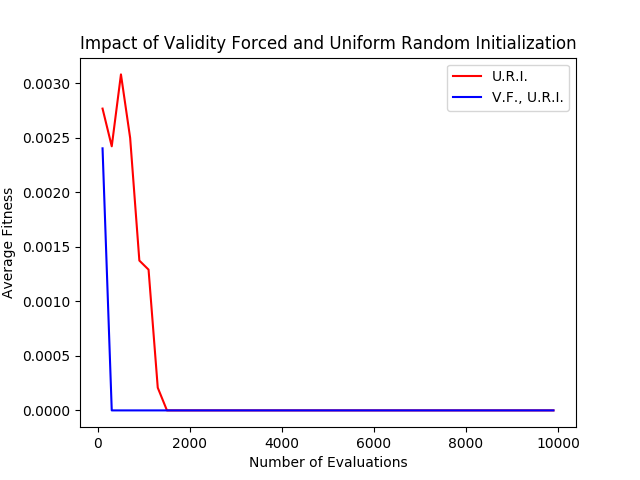
\includegraphics[scale=0.4]{q2_random_board_basic_ur_vs_vfur.png}
		% \caption{Assigned Board}
		\end{figure}
		\begin{center}
		\begin{tabular}{ || c | c | c | c ||}
		\hline
		       & F.V. and U.R. & U.R.\\ 
		 \hline\hline
		 Average & 0.0002730228525 &	0.00004809653916 \\ 
		 \hline
		 Standard Deviation &	0.0007716248776 &	0.0003400938899\\
		 \hline
		 variance &	0.0000005954049518 &	0.000000115663854 \\
		 \hline
		 T-test &	0.06359168534	& \\
		 \hline
		\end{tabular}
		\end{center}
\clearpage
		
		\subsubsection{Penalty Fitness}
			Given the p-value of the T-test, both configurations performed equivalently.
			\begin{figure}[!htb]
			\centering
			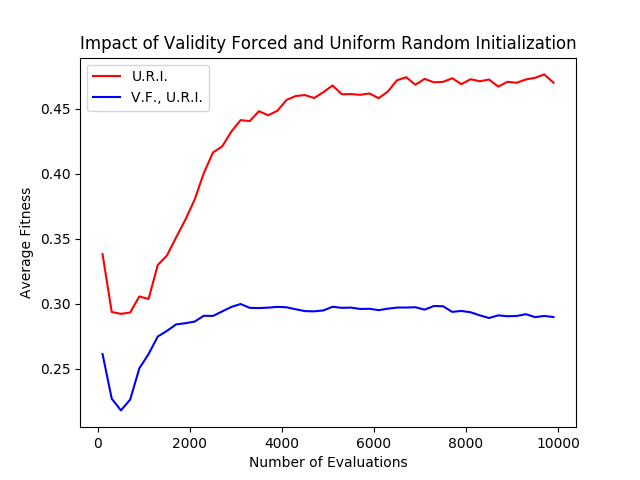
\includegraphics[scale=0.4]{q2_random_board_penalty_ur_vs_vfur.png}
			% \caption{Assigned Board}
			\end{figure}
			\begin{center}
			\begin{tabular}{ || c | c | c | c ||}
			\hline
			       & F.V. and U.R. & U.R.\\ 
			 \hline\hline
			 Average & 0.4299146547	& 0.2870118415 \\ 
			 \hline
			 Standard Deviation &	0.05929583822 &	0.01890259673\\
			 \hline
			 variance &	0.00351599643 &	0.000357308163 \\
			 \hline
			 T-test &	0	& \\
			 \hline
			\end{tabular}
			\end{center}
	
	
		\subsubsection{Repair Fitness}
			Both configurations were equivalent. Repair fitness functions similarly to non-random
			initialization.
			\begin{figure}[!htb]
			\centering
			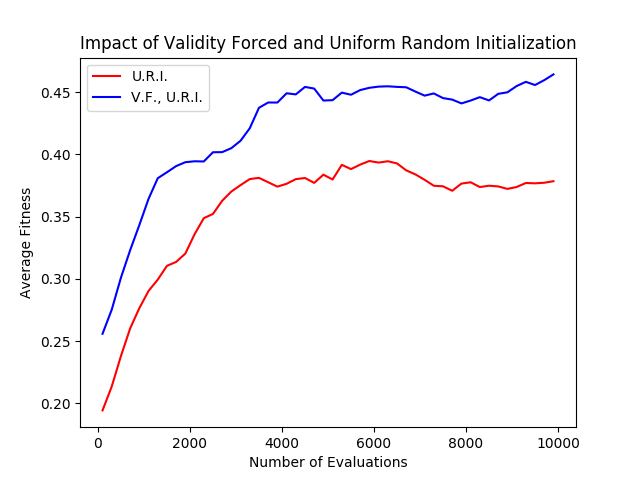
\includegraphics[scale=0.4]{q2_random_board_repair_ur_vs_vfur.png}
			% \caption{Assigned Board}
			\end{figure}
			\begin{center}
			\begin{tabular}{ || c | c | c | c ||}
			\hline
			       & F.V. and U.R. & U.R.\\ 
			 \hline\hline
			 Average & 0.3561276062 &	0.4215879912 \\ 
			 \hline
			 Standard Deviation &	0.04777985977 &	0.0488061994\\
			 \hline
			 variance &	0.002282915 &	0.0023820451 \\
			 \hline
			 T-test &	0.0000000009247323641		& \\
			 \hline
			\end{tabular}
			\end{center}


\section{Penalty Function Coefficient Effects on Solution Quality}
	\subsection{Assigned Board}
		A constraint-satisfaction EA employing different penalty coefficients preform at different levels. Considering the T-test comparing values 0.5 and 1.0, it is clear from the p-value of 0.005 that the latter preforms better. Although, when comparing values 1.0 and 1.5 the performance is similar. Overall, The value of the penalty 		coefficient is positively correlated to solution quality to a point, where the coefficient stops mattering and the EA is basically operating with only valid individuals.
		
		\begin{figure}[!htb]
		\centering
		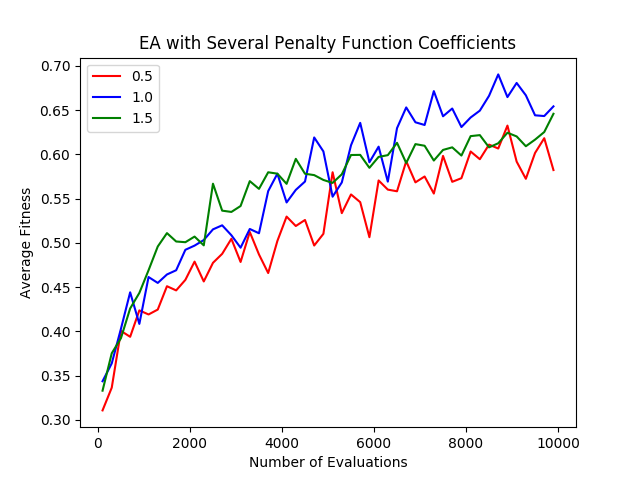
\includegraphics[scale=0.4]{q3_assigned_board.png}
		% \caption{Assigned Board}
		\end{figure}
		
		
		\begin{center}
		\begin{tabular}{ || c | c | c | c ||}
		\hline
		       & P.C. = 0.5 & P.C. = 1.0 & P.C. = 1.5 \\ 
		 \hline\hline
		 Average & 0.5189377027 &	0.5656762162 &	0.5592304054	 \\ 
		 \hline
		 Standard Deviation &	0.07416746452 &	0.08893047016 &	0.06975757603	 \\
		 \hline
		 variance &	0.005500812794 &	0.007908628523 &	0.004866119414 \\
		 \hline
		 T-test &	0.005300537023	& &	0.687684336 \\
		 \hline
		\end{tabular}
		\end{center}
	
\clearpage
	\subsection{Random Boards}
		Considering the T-test comparing values 0.5 and 1.0, the p-value is greater than alpha, so, both samples preform equivalently. The same situation occurs with values 1.0 and 1.5. Overall, all values preformed similarly on the random boards, considering the assigned board's results this may indicate that random boards could use a 	slightly higher coefficient to see any performance differences.
		
		\begin{figure}[!htb]
		\centering
		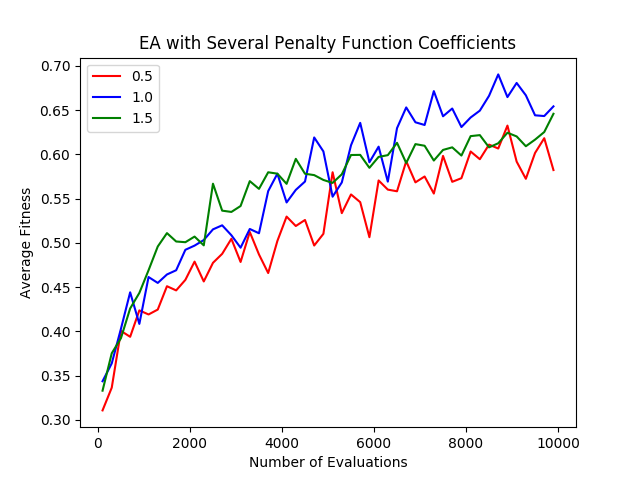
\includegraphics[scale=0.4]{q3_random_board.png}
		% \caption{Assigned Board}
		\end{figure}
		
		\begin{center}
		\begin{tabular}{ || c | c | c | c ||}
		\hline
		       & P.C. = 0.5 & P.C. = 1.0 & P.C. = 1.5 \\ 
		 \hline\hline
		 Average & 0.7081163989 &	0.7104515572 &	0.7232313518	 \\ 
		 \hline
		 Standard Deviation &	0.06341326214 &	0.05701996763 &	0.05999335936	 \\
		 \hline
		 variance &	0.004021241816 &	0.003251276708 &	0.003599203167 \\
		 \hline
		 T-test &	0.8468756373 &	&	0.2775989777 \\
		 \hline
		\end{tabular}
		\end{center}
		
		\end{document}